\documentclass[a4paper, 11pt]{article}

\usepackage[french]{babel}
\usepackage[french, noheader]{packages/sleek}
\usepackage[nomessages]{fp}
\usepackage{packages/sleek-title}
\usepackage{tabularx}
\usepackage{tikz}
\usetikzlibrary{arrows.meta, positioning, calc}

\addbibresource{references.bib}
\setcounter{tocdepth}{1}
\setlength{\emergencystretch}{3em}

\newcommand{\Mzero}{M0}
\newcommand{\dAUC}{$\Delta$AUC}
\newcolumntype{Y}{>{\raggedright\arraybackslash}X}

\title{Que voit un détecteur de musique IA~?\\[0.4em]
{\Large Réplication de travaux publiés, sans musique générée à l'entraînement}}
\author{Cédric \textsc{Dada}}
\date{22 novembre 2026}

\begin{document}

\maketitle

\section*{Résumé}

Ce projet reprend trois travaux de Deezer et vérifie si leurs résultats tiennent dans un autre cadre. Afchar et
al. entraînent un détecteur à reconnaître la reconstruction de musique réelle par des auto-encodeurs
\cite{afchar2024easy, afchar2025challenges}. La même équipe explique les artefacts de ces décodeurs par
l'analyse de Fourier \cite{afchar2025fourier}, et Dugelay et al. rendent le détecteur robuste aux changements de
vitesse \cite{dugelay2026robustness}. Ici, aucune musique générée ne sert à l'entraînement : quatre détecteurs
apprennent à distinguer 2\,000 pistes de la Free Music Archive (FMA) de leur reconstruction par EnCodec 24~kHz,
puis sont testés sur les cinq générateurs de FakeMusicCaps.

Deux résultats tiennent. Le premier concerne la cadence du décodeur. Le détecteur à fakeprint apprend un peigne
de pics espacés de 75~Hz, la cadence d'EnCodec 24~kHz, alors que MusicGen laisse un peigne espacé de 50~Hz ;
MusicGen n'est pas mieux détecté que les autres générateurs (écart de $-0{,}041$, IC~95~\%
$[-0{,}052~;~-0{,}029]$). Une expérience ajoutée après ces premiers résultats teste ce point directement :
entraîné sur l'EnCodec 32~kHz de MusicGen, le même détecteur apprend un peigne à 50~Hz et passe de 0,796 à 0,997
d'AUC sur MusicGen ($+0{,}200$ $[+0{,}183~;~+0{,}217]$). Il progresse aussi sur les autres générateurs, et son
débit plus faible (2,2~kbit/s) reste un facteur confondu. Le second résultat concerne la robustesse. Sous un
changement de vitesse de 10~\%, le fakeprint linéaire tombe au hasard (AUC de 0,796 à 0,499), tandis que la
version log-fréquence de Dugelay et al. ne perd rien, ni sous la vitesse ni sous un MP3 à 128~kbit/s.

Le transfert vers les générateurs, en revanche, ne peut pas être établi avec ce protocole. FakeMusicCaps ne
contient pas les vrais extraits MusicCaps : les négatifs sont donc des morceaux FMA. Un détecteur trivial, qui ne
voit que des descripteurs de format (bande passante, niveau, silences), atteint des AUC du même ordre que le
fakeprint (0,61 à 0,97, contre 0,62 à 0,94). C'est la principale limite de l'étude.

\vspace{1em}
\tableofcontents
\newpage

% =====================================================================================================
\section{Introduction}

Les générateurs de musique à partir de texte (MusicGen, Stable Audio Open, AudioLDM2\dots) produisent des
extraits difficiles à distinguer à l'oreille. Afchar et al. proposent une façon de les détecter sans dépendre
d'un générateur donné : entraîner le détecteur à reconnaître la \emph{reconstruction} d'une piste réelle par un
auto-encodeur neuronal \cite{afchar2024easy, afchar2025challenges}. L'idée repose sur un constat : beaucoup de
générateurs produisent leur signal avec un décodeur neuronal, et ces décodeurs laissent des artefacts spectraux
réguliers, en particulier des pics dus au suréchantillonnage par convolutions transposées
\cite{pons2021upsampling, afchar2025fourier}.

Ce rapport ne propose pas de nouvelle méthode. Il reprend ces travaux dans un autre cadre et mesure ce qui
tient. Le cadre diffère sur trois points : aucun morceau généré n'est utilisé à l'entraînement, même pour le
détecteur robuste de Dugelay et al. \cite{dugelay2026robustness} ; le test porte sur cinq générateurs open
source réunis dans FakeMusicCaps ; un détecteur trivial et un codec identité servent de contrôles. Un résultat
qui ne tiendrait que sur les données d'origine (Suno, Udio, reconstructions de FMA \emph{medium}) devrait
apparaître dans ce changement de cadre.

Un détecteur n'apprend que ce qui sépare ses deux classes, et rien ne garantit que ce soit l'artefact visé. C'est
le problème des \emph{raccourcis} \cite{geirhos2020shortcut}. Il est central ici, car notre protocole de test
oppose deux bases de données différentes (section~\ref{sec:donnees}).

% =====================================================================================================
\section{Ce que disent les papiers}
\label{sec:papiers}

Chaque affirmation ci-dessous a été relue dans le papier (version HTML d'arXiv). La section du papier est
indiquée entre parenthèses.

\subsection{Détecter des reconstructions d'auto-encodeurs (Afchar et al., 2024 et 2025)}

Afchar et al. \cite{afchar2024easy} entraînent un CNN (six couches de convolution, environ 1,6~million de
paramètres) sur des spectrogrammes d'amplitude (§2.3). Les exemples réels viennent du sous-ensemble
\emph{medium} de FMA (25\,000 pistes). Les faux sont leurs reconstructions par Encodec, DAC, le décodeur de
Musika et une reconstruction mel suivie de Griffin-Lim (§2.1--2.2). Le papier discute le risque de
confusion entre artefact et format (« \emph{confounding} ») : les reconstructions sont enregistrées au même
débit que l'original (§2.1).

Trois résultats concernent ce projet. Le transfert entre débits d'un même codec est bon (par exemple d'Encodec
24 vers 6 et 3), mais la généralisation à une autre famille d'auto-encodeurs est « presque toujours nulle »
(§3.2). Les performances chutent fortement sous changement de hauteur ($\pm 2$ demi-tons), ajout de bruit blanc
et ré-encodage MP3, AAC ou Opus à 64~kbit/s ; elles résistent à l'étirement temporel (80 à 120~\%), à
l'égalisation et à la réverbération (§3.1). Ce papier ne teste aucun générateur réel.

La version ICASSP 2025 \cite{afchar2025challenges} reprend l'approche et coupe le spectre à 16~kHz pour ne pas
s'appuyer sur des artefacts de conversion MP3 (§II-B, note~8). Elle teste le détecteur sur 50 pistes générées
par MusicGen à partir de prompts et rapporte un score de détection de 99,9~\% (§II-D). Elle précise aussi que
les probabilités produites ne doivent pas être prises au pied de la lettre (§III-C). Le README du dépôt
\texttt{deezer/deepfake-detector} indique qu'entraîner seulement sur des auto-encodeurs permet de détecter de la
musique entièrement générée à partir de prompts, sans nommer de générateur.

\subsection{Une explication de Fourier des artefacts (Afchar et al., ISMIR 2025)}
\label{sec:fourier}

Afchar et al. \cite{afchar2025fourier} montrent qu'une convolution transposée périodise le spectre : des pics
apparaissent à chaque multiple de la fréquence d'échantillonnage $f_s$ de la couche (§3.2). Ces artefacts sont
« inhérents à l'architecture choisie plutôt qu'une conséquence des données d'entraînement ou des poids »
(résumé). La vérification empirique porte sur DAC : deux graines d'entraînement et plusieurs jeux de données
donnent les mêmes pics (§4.2). Le papier donne l'exemple d'EnCodec, dont les pas de suréchantillonnage
$\{8, 5, 4, 2\}$ créent 161 pics (§3.3).

L'empreinte (\emph{artifact fingerprint}, appelée \emph{fakeprint} par Dugelay et al.) s'obtient en soustrayant
au spectre moyen ses minima locaux sur une fenêtre glissante (§4.1). Une régression logistique d'environ 10\,000
paramètres sur cette empreinte distingue les pistes FMA de leurs reconstructions par DAC, Encodec et Musika avec
plus de 99,6~\% de précision (§4.3, tableau~1). Sur des chansons Suno et Udio (données SONICS, avec FMA comme
classe réelle), la précision approche 100~\%, sauf sur Udio~32, non vu à l'entraînement (39,8~\%). Le papier
n'étudie pas la robustesse aux manipulations ; il anticipe que celles qui déplacent les fréquences
(rééchantillonnage, changement de hauteur) affecteront le modèle (conclusion).

Le papier ne mentionne ni MusicGen, ni la cadence en hertz des trames d'EnCodec. Le lien avec 75~Hz est notre
calcul : le produit des pas vaut $8 \times 5 \times 4 \times 2 = 320$, et $24\,000 / 320 = 75$~Hz.

\subsection{Un détecteur robuste aux changements de vitesse (Dugelay et al., ISMIR 2026)}

Dugelay et al. \cite{dugelay2026robustness} montrent que le détecteur linéaire d'Afchar et al. s'effondre sous
changement de vitesse et de hauteur, car tout le fakeprint se déplace en bloc (§4.1, §6.2). Leur méthode
interpole le fakeprint sur une grille géométrique (1\,920 cases par octave, §5.2), où un changement de vitesse
devient une translation (§3.4). Un unique filtre appris est corrélé à ce fakeprint, puis on prend le maximum
sur les décalages (§4.2). Ils entraînent sur 5\,000 pistes Suno~v5 contre 5\,000 pistes de FMA-small, et aussi
sur Suno~v3.5 et Udio~v120 issus de SONICS (§5.1). Dans la condition « attaque », l'entraînement utilise des
facteurs de vitesse tirés entre $\times$0,7 et $\times$1,4, pour leur modèle comme pour le modèle d'Afchar et
al. (§5.1). Ils écrivent que d'autres manipulations courantes, dont la compression par codec, « restent non
testées » (§6.3), et que le modèle ne généralise pas à d'autres générateurs que ceux d'entraînement (§6.3).

\subsection{Raccourcis en détection audio}

Geirhos et al. définissent un raccourci comme une règle de décision qui marche sur le banc d'essai habituel
mais ne se transfère pas à des conditions plus difficiles \cite{geirhos2020shortcut}. En détection de voix
synthétique, Müller et al. montrent qu'un classifieur qui ne voit que la durée du silence initial obtient un
taux d'égale erreur de 15~\% sur l'évaluation d'ASVspoof~2019~LA, contre 50~\% au hasard (§5.1, tableau~1)
\cite{muller2021silence}. Dans un second papier, des modèles entraînés sur ASVspoof voient leur taux d'erreur
multiplié par 2 à 10 sur des enregistrements réels (§5.3) \cite{muller2022generalize}. Des jeux récents
sont construits pour limiter ces raccourcis : Echoes \cite{pascu2026echoes} aligne chaque morceau généré sur un
morceau réel de FMA, en conditionnant la génération sur l'audio réel ou sur une description de la chanson
(résumé, §II-A).

% =====================================================================================================
\section{Questions de réplication}
\label{sec:questions}

\paragraph{Q1. Un détecteur entraîné sur des reconstructions de codec détecte-t-il de vrais générateurs~?}
Afchar et al. rapportent 99,9~\% de détection sur 50 pistes MusicGen \cite{afchar2025challenges}, mais une
généralisation quasi nulle entre familles d'auto-encodeurs \cite{afchar2024easy}. On mesure si des détecteurs
entraînés sur FMA et FMA-EnCodec détectent les cinq générateurs de FakeMusicCaps.

\paragraph{Q2. Les artefacts dépendent-ils de l'architecture du décodeur, et en particulier de sa cadence~?}
Afchar et al. montrent que les pics dépendent de l'architecture et pas des poids \cite{afchar2025fourier}.
D'après notre calcul (section~\ref{sec:fourier}), un détecteur appris sur EnCodec 24~kHz (75 trames par
seconde) devrait voir un peigne espacé de 75~Hz. MusicGen utilise un EnCodec à 32~kHz et 50 trames par seconde \cite{copet2023musicgen}, donc un peigne
espacé de 50~Hz. Partager le « même codec » ne garantit donc pas que MusicGen soit mieux détecté. On mesure les
poids appris, le peigne laissé par chaque générateur et l'écart de détection entre MusicGen et les autres. Après
ces premières mesures, on a ajouté un test direct : entraîner M1 sur l'EnCodec 32~kHz de MusicGen (« oracle »).

\paragraph{Q3. Une partie de la performance vient-elle de raccourcis de format~?} La littérature sur les
raccourcis \cite{geirhos2020shortcut, muller2021silence, muller2022generalize} montre qu'un détecteur peut
s'appuyer sur des différences de format. On mesure ce qu'obtient un détecteur trivial qui ne voit que de telles
différences.

\paragraph{Q4. Le fakeprint linéaire s'effondre-t-il sous changement de vitesse, et la log-fréquence
résiste-t-elle~?} Dugelay et al. le montrent avec des modèles entraînés sur de la musique générée
\cite{dugelay2026robustness}. On mesure si cela tient quand le détecteur log-fréquence est entraîné uniquement
sur des reconstructions EnCodec, et on ajoute le MP3 à 128~kbit/s, qu'ils n'ont pas testé.

% =====================================================================================================
\section{Protocole}
\label{sec:protocole}

\subsection{Données}
\label{sec:donnees}

\paragraph{FMA.} 2\,000 pistes du sous-ensemble \emph{small} de la Free Music Archive
\cite{defferrard2017fma} (une est illisible, il en reste 1\,999), issues de 1\,047 artistes et réparties en huit
genres. Le découpage en apprentissage, validation et test (70/10/20~\%) se fait par artiste. Chaque
piste donne deux segments de 10~s, soit 2\,888 paires en apprentissage, 378 en validation et 732 en test
(366 pistes, 210 artistes).

\paragraph{FakeMusicCaps.} FakeMusicCaps \cite{comanducci2024fakemusiccaps} regroupe 27\,605 extraits de 10~s,
mono, à 16~kHz, produits par cinq modèles à partir des légendes de MusicCaps \cite{agostinelli2023musiclm}
(§III-A, §III-B), soit 5\,521 par générateur. Les cinq générateurs ont reçu les mêmes légendes, ce qui permet
d'apparier les comparaisons entre générateurs. L'archive téléchargée ne contient pas les extraits réels de
MusicCaps : \textbf{les négatifs de chaque test FakeMusicCaps sont donc les 732 segments réels du test FMA}. Un
test \texttt{fmc:<générateur>} oppose ainsi des fichiers FakeMusicCaps à des fichiers FMA, pas seulement du
généré à du réel. C'est un choix de ce protocole, pas une propriété des méthodes répliquées.

\begin{table}[h]
    \centering
    \small
    \begin{tabularx}{\textwidth}{lY}
        \toprule
        Générateur & Décodeur \\
        \midrule
        MusicGen (medium) & EnCodec 32~kHz, 50 trames par seconde \cite{copet2023musicgen} \\
        Stable Audio Open & auto-encodeur variationnel sur forme d'onde \cite{evans2024stableaudioopen} \\
        AudioLDM2 (\texttt{audioldm2-music}) & VAE sur spectrogramme mel, vocodeur HiFi-GAN \cite{liu2024audioldm2} \\
        MusicLDM & VAE sur spectrogramme mel, vocodeur HiFi-GAN ré-entraîné sur de la musique \cite{chen2023musicldm} \\
        Mustango & VAE d'AudioLDM \cite{melechovsky2024mustango} ; vocodeur non nommé dans la description du
        modèle ; Tango, dont Mustango reprend l'architecture en ajoutant le module MuNet, utilise le HiFi-GAN
        d'AudioLDM \cite{ghosal2023tango} \\
        \bottomrule
    \end{tabularx}
    \caption{Décodeurs des générateurs de FakeMusicCaps, d'après leurs papiers.}
    \label{tab:decodeurs}
\end{table}

\subsection{Chaîne de normalisation commune}

L'objectif de la chaîne (figure~\ref{fig:chaine}) est que la seule différence entre un segment réel et son faux
soit le passage par le codec. Chaque piste FMA est décodée en mono à sa fréquence native. La branche « faux »
passe à 24~kHz, traverse EnCodec \cite{defossez2022encodec} (6 ou 12~kbit/s), puis redescend à 16~kHz, la
fréquence de FakeMusicCaps. La branche « réel » subit le même aller-retour de rééchantillonnage, sans le codec.
Le faux est aligné sur le réel par corrélation croisée (retard estimé entre $-1$ et 2 échantillons). Les deux
sont découpés aux mêmes instants et normalisés au même niveau RMS ($-23$~dBFS, avec un limiteur de crête
déclenché sur 0,56~\% des segments). Les extraits FakeMusicCaps ne passent que par la découpe et la
normalisation de niveau.

Un contrôle négatif vérifie la chaîne : un « codec identité » produit des faux qui ne diffèrent des réels que
par le traitement commun. Tout détecteur doit y obtenir une AUC de 0,5.

Pour l'oracle MusicGen (section~\ref{sec:peigne}), la branche « faux » passe à 32~kHz par l'EnCodec de MusicGen.
Les réels appariés restent ceux de l'aller-retour à 24~kHz, à l'entraînement comme au test : l'oracle voit donc
exactement les mêmes négatifs que les autres détecteurs.

\begin{figure}[h]
\centering
\begin{tikzpicture}[
    box/.style={draw, rounded corners=2pt, align=center, font=\small, inner sep=4pt, minimum height=2.2em},
    arr/.style={-{Stealth[length=2mm]}, thick},
    node distance=0.5cm and 0.55cm]
    \node[box] (fma) {Piste FMA\\MP3, 30~s};
    \node[box, right=of fma, yshift=0.75cm] (fake) {EnCodec 24~kHz\\(6 ou 12~kbit/s) $\to$ 16~kHz};
    \node[box, right=of fma, yshift=-0.75cm] (real) {aller-retour\\24~kHz $\to$ 16~kHz};
    \node[box, right=of fake, yshift=-0.75cm] (chain) {alignement, 2 segments\\de 10~s, RMS $-23$~dBFS};
    \node[box, right=of chain] (train) {Entraînement\\M0 à M3};
    \node[box, below=1.2cm of fma] (fmc) {FakeMusicCaps\\WAV 16~kHz, 10~s};
    \node[box, right=of fmc, xshift=2.6cm] (lvl) {même découpe et\\même niveau RMS};
    \node[box, right=of lvl] (test) {Test \texttt{fmc:<gén.>}\\5\,521 faux / 732 réels};
    \draw[arr] (fma) -- (fake);
    \draw[arr] (fma) -- (real);
    \draw[arr] (fake) -- (chain);
    \draw[arr] (real) -- (chain);
    \draw[arr] (chain) -- (train);
    \draw[arr] (fmc) -- (lvl);
    \draw[arr] (lvl) -- (test);
    \draw[arr, dashed] (chain.south) -- node[right, font=\footnotesize, align=left] {réels du\\split test} (test.north west);
\end{tikzpicture}
\caption{Chaîne de traitement. En haut, les paires d'apprentissage : la branche réelle subit le même
aller-retour de rééchantillonnage que la branche faux, sans le codec. En bas, les tests FakeMusicCaps, dont
les négatifs sont les segments réels du test FMA.}
\label{fig:chaine}
\end{figure}

\subsection{Détecteurs}

Quatre détecteurs sont entraînés uniquement sur les paires FMA réel / FMA-EnCodec ; un cinquième est
pré-entraîné (tableau~\ref{tab:detecteurs}). M2 et M3 sont entraînés avec trois graines ; M0 et M1 sont
déterministes. M1 est aussi entraîné une fois sur des reconstructions par l'EnCodec 32~kHz de MusicGen
(« oracle », section~\ref{sec:peigne}).

\begin{table}[h]
    \centering
    \small
    \begin{tabularx}{\textwidth}{lYY}
        \toprule
        & Entrée et modèle & Rôle \\
        \midrule
        M0 & descripteurs triviaux après la chaîne (fréquence de coupure à 85 et 95~\%, RMS, silences de
        début et de fin, plancher de bruit, écrêtage, composante continue) ; gradient boosting & contrôle :
        détecteur de raccourcis \\
        M1 & fakeprint linéaire (TFD de 8\,192 points, bande 1--8~kHz) ; régression logistique & reprise de
        \cite{afchar2025fourier} \\
        M2 & spectrogramme en dB (0--8~kHz) ; petit CNN 1D, recadrages de 5~s & modèle appris de bout en bout \\
        M3 & fakeprint en log-fréquence (1\,920 cases par octave) ; corrélation croisée avec un filtre appris
        puis maximum ; augmentation par changement de vitesse ($\times$0,7 à $\times$1,4) & reprise de
        \cite{dugelay2026robustness} \\
        M4 & SONICS SpecTTTra, pré-entraîné sur des chansons Suno et Udio, inférence seule & référence externe
        \cite{rahman2025sonics} \\
        \bottomrule
    \end{tabularx}
    \caption{Les cinq détecteurs. M3 combine deux mécanismes de robustesse, l'architecture log-fréquence et
    l'augmentation par vitesse, que cette étude ne sépare pas.}
    \label{tab:detecteurs}
\end{table}

\subsection{Évaluation}

\paragraph{Mesures.} La mesure principale est l'aire sous la courbe ROC (AUC) : 0,5 pour un détecteur au
hasard, 1 pour une séparation parfaite. On rapporte aussi le taux de détection (TPR) et de faux positifs (FPR) à
un seuil fixé une fois pour toutes sur la validation (1~\% de faux positifs sur les segments réels), ainsi que
l'erreur de calibration (ECE) \cite{guo2017calibration}.

\paragraph{Intervalles de confiance.} Les segments d'un même artiste, ou les extraits d'une même légende, ne
sont pas indépendants. Les intervalles à 95~\% sont obtenus par bootstrap groupé
\cite{efron1993bootstrap} : on tire avec remise des artistes (FMA) et des légendes (FakeMusicCaps), 1\,000 fois.
Le même tirage des groupes sert à toutes les séries. Deux AUC calculées sur des segments qui partagent
des groupes sont donc comparées de façon appariée : deux détecteurs, deux générateurs (les légendes sont
communes) ou un même jeu avant et après attaque.

\paragraph{Comparaisons principales.} Quatre comparaisons résument les questions Q2 à Q4 (détecteurs entraînés
à 6~kbit/s, M3 graine~1) : l'écart d'AUC de M1 entre MusicGen et la moyenne des quatre autres générateurs ;
l'AUC de M0 sur MusicGen face à 0,5 ; l'écart apparié M1 $-$ M0 sur MusicGen ; l'écart apparié
\dAUC(M1) $-$ \dAUC(M3) sous vitesse $\times$1,1. Leurs valeurs $p$ sont bilatérales, obtenues par inversion de
l'intervalle percentile, et corrigées ensemble par la méthode de Holm \cite{holm1979}. Avec 1\,000 tirages, la
plus petite valeur $p$ bilatérale possible est $2/1001 \approx 0{,}002$.

\paragraph{Graines.} Pour M2 et M3, la variabilité entre graines est rapportée \emph{séparément} des
intervalles bootstrap : ce sont deux sources d'incertitude différentes.

\paragraph{Attaques.} Trois attaques sont appliquées au test MusicGen : changement de vitesse $\times$0,9 et
$\times$1,1 par rééchantillonnage, qui modifie à la fois le tempo et la hauteur, donc multiplie toutes les
fréquences ; aller-retour MP3 à 128~kbit/s. Elles touchent réels et faux, et le seuil n'est pas réajusté. M1,
M3 et M2 (graine~1) sont évalués sur exactement les mêmes segments.

% =====================================================================================================
\section{Résultats}

\subsection{Contrôles : la chaîne ne fuit pas}

Sur leur propre domaine (FMA contre FMA-EnCodec, artistes jamais vus), les détecteurs appris séparent presque
parfaitement les deux classes : AUC de 1,000 pour M1, de 0,996 à 0,999 pour M2 et M3. Passer d'un débit à
l'autre (6 vers 12~kbit/s et inversement) ne coûte rien, comme le transfert entre débits observé par Afchar et
al. \cite{afchar2024easy}. Sur le contrôle identité, tous les détecteurs obtiennent 0,500 : aucun
artefact de traitement ne distingue les deux branches. M0 obtient 0,849 sur son domaine, ce qui est attendu : le
codec réduit réellement la bande passante, et M0 la mesure. M4, entraîné sur d'autres générateurs, reconnaît mal
les reconstructions EnCodec (0,563).

\begin{figure}[h]
    \centering
    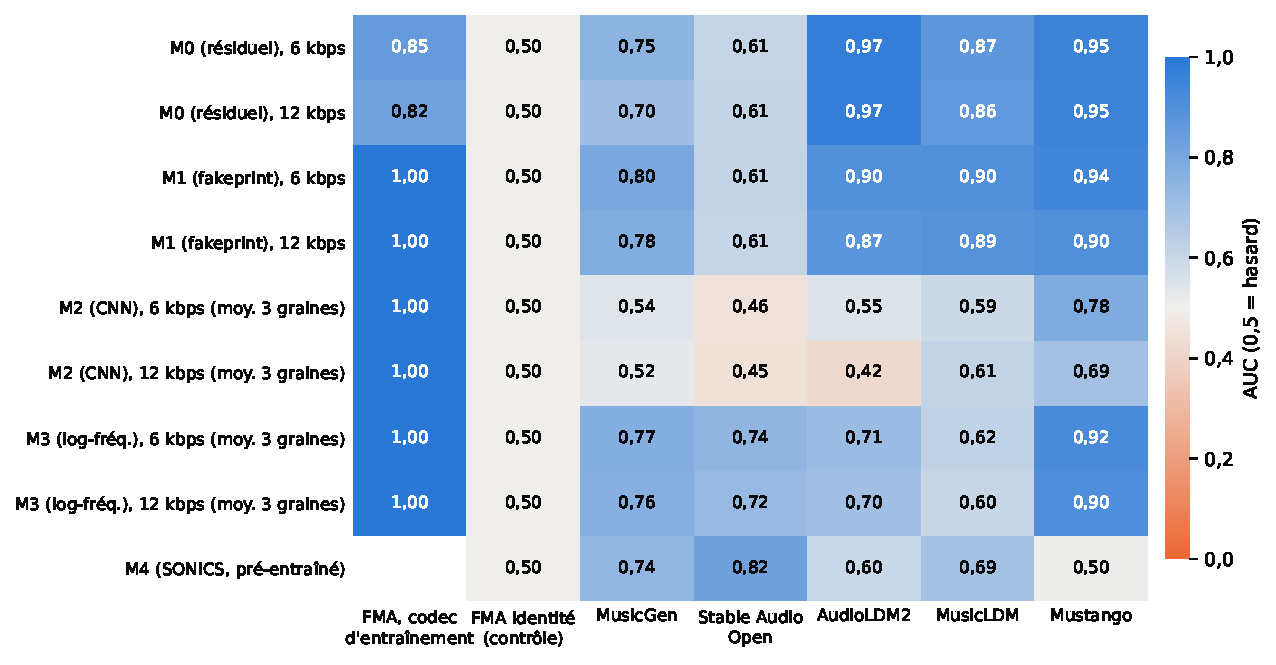
\includegraphics[width=\textwidth]{figures/fig_matrice_auc.pdf}
    \caption{Matrice de généralisation. AUC par détecteur et jeu de test ; pour M2 et M3, moyenne des trois
    graines. Orange : en dessous du hasard. La première colonne est le test sur le domaine d'entraînement,
    la deuxième le contrôle identité.}
    \label{fig:matrice}
\end{figure}

\subsection{Q1 : transfert vers les générateurs}

La figure~\ref{fig:matrice} rassemble toutes les AUC. M1 entraîné à 6~kbit/s obtient 0,796 $[0{,}779~;~0{,}814]$
sur MusicGen, 0,896 sur AudioLDM2, 0,899 sur MusicLDM et 0,938 sur Mustango ; Stable Audio Open est le plus
difficile (0,615). M3 va de 0,62 à 0,92 selon le générateur. M2 est instable : sur MusicGen, ses trois graines
donnent 0,444, 0,611 et 0,576 à 6~kbit/s, et l'écart-type entre graines atteint 0,25 sur Stable Audio Open à
12~kbit/s, plus que la largeur des intervalles bootstrap (annexe~\ref{app:graines}).

Ces AUC ne se traduisent pas en détections au seuil fixé. Pour M1, le taux de détection à 1~\% de faux positifs
n'est que de 34~\% sur MusicGen, 11~\% sur AudioLDM2, 10~\% sur MusicLDM, 15~\% sur Mustango et 1,7~\% sur
Stable Audio Open. Le FPR observé sur les réels reste à 0,5~\%. Les scores des faux FakeMusicCaps sont bien
ordonnés mais beaucoup plus bas que ceux des faux d'entraînement, et la calibration est mauvaise (ECE de 0,71 à
0,85).

\paragraph{Comparaison avec les papiers.} Le score de 99,9~\% rapporté par Afchar et al. sur 50 pistes MusicGen
\cite{afchar2025challenges} n'est pas retrouvé ici. Au seuil fixé, M1 détecte 34~\% des extraits MusicGen, et
M2, le plus proche de leur CNN, obtient une AUC de 0,44 à 0,61 selon la graine. Ce n'est pas une réfutation :
les détecteurs, les données d'entraînement, les extraits MusicGen et la mesure diffèrent. Le résultat ne se
transpose simplement pas tel quel à ce cadre. Dans l'autre sens, nos AUC de 0,90 à 0,94 sur les trois
générateurs à vocodeur sembleraient contredire la généralisation quasi nulle entre familles observée en 2024
\cite{afchar2024easy}, mais Q3 montre qu'elles s'expliquent en grande partie par un raccourci.

\paragraph{Verdict.} Transfert apparent, \textbf{impossible à séparer du raccourci avec ce protocole}.

\subsection{Q2 : un peigne à la cadence du codec d'entraînement}
\label{sec:peigne}

Pour chaque source, on calcule l'empreinte moyenne de 300 segments et on lui soustrait celle des réels FMA. On
mesure ensuite le \emph{contraste de peigne} du profil obtenu : la valeur moyenne, en écarts-types du profil,
aux multiples d'un espacement $s$ donné. C'est une mesure descriptive, définie pour cette analyse, sans
intervalle de confiance. D'après l'explication de Fourier, un décodeur qui suréchantillonne à cadence de trame
fixe doit donner un contraste élevé quand $s$ est cette cadence ou l'un de ses multiples.

\begin{figure}[h]
    \centering
    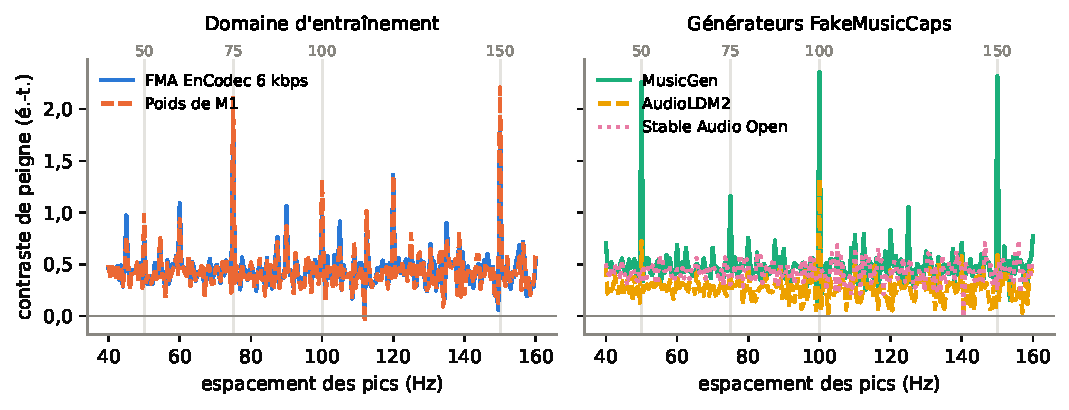
\includegraphics[width=\textwidth]{figures/fig_peigne.pdf}
    \caption{Contraste de peigne en fonction de l'espacement des pics. À gauche, l'empreinte des
    reconstructions EnCodec (moins celle des réels) et les poids de la régression logistique de M1 : tous
    deux culminent à 75 et 150~Hz. À droite, les générateurs : MusicGen culmine à 50, 100 et 150~Hz,
    AudioLDM2 montre un pic faible à 100~Hz, Stable Audio Open aucun. 300 segments par série ; mesure
    descriptive, sans intervalle de confiance.}
    \label{fig:peigne}
\end{figure}

M1 a appris l'artefact du codec (figure~\ref{fig:peigne}) : ses douze plus grands poids tombent sur des
multiples de 75~Hz (2\,400, 3\,600, 4\,800, 6\,000, 7\,200~Hz\dots), et le contraste de peigne de ses poids vaut
2,11 à 75~Hz contre 0,97 à 50~Hz. MusicGen, lui, laisse un peigne espacé de 50~Hz (contraste 2,26 à 50~Hz, 1,16
à 75~Hz), ce qui correspond aux 50 trames par seconde de son EnCodec à 32~kHz. Les deux peignes ne
coïncident qu'aux multiples de 150~Hz : M1 ne voit qu'une partie de l'artefact de MusicGen. Stable Audio Open ne
laisse aucun peigne visible et c'est le générateur le plus difficile pour tous les détecteurs. AudioLDM2 n'a
qu'un peigne faible, à 100~Hz, et il est pourtant parmi les mieux détectés, ce qui renvoie à Q3.

Partager le codec ne suffit donc pas. L'écart d'AUC entre MusicGen et la moyenne des quatre autres vaut
$-0{,}041$ $[-0{,}052~;~-0{,}029]$ à 6~kbit/s ($p$ corrigé $= 0{,}008$) et $-0{,}041$
$[-0{,}053~;~-0{,}029]$ à 12~kbit/s. Cet écart n'est pas seulement dû au peigne : M0 classe aussi MusicGen
parmi les générateurs difficiles (Q3). Parmi les détecteurs appris sur EnCodec 24~kHz, M3 est le seul qui
favorise légèrement MusicGen : l'écart vaut de $+0{,}014$ à $+0{,}037$ selon la graine et le débit, avec des
intervalles qui excluent tous zéro (annexe~\ref{app:graines}). L'effet est faible, et Mustango reste mieux
détecté (0,92 contre 0,77).

\paragraph{Oracle MusicGen.} Cette expérience a été ajoutée après les résultats ci-dessus. On l'appelle
« oracle » parce qu'elle utilise une information qu'on n'aurait pas face à un générateur inconnu : son décodeur
exact. M1 est ré-entraîné à l'identique, mais ses faux sont les pistes FMA reconstruites par l'EnCodec 32~kHz
de MusicGen (poids de \texttt{musicgen-small} : 50 trames par seconde et 2,2~kbit/s, soit 4 dictionnaires, le
débit par défaut de ce modèle). Les négatifs restent les mêmes segments réels, ce qui permet des comparaisons
appariées avec M1 entraîné à 6~kbit/s. Ces comparaisons ne font pas partie de la correction de Holm.

Les reconstructions FMA par ce codec laissent le même peigne que MusicGen : contraste de 2,31 à 50~Hz et de
1,28 à 75~Hz, contre 2,26 et 1,16 pour MusicGen (figure~\ref{fig:peigne_oracle}). Les poids de l'oracle
suivent : ses douze plus grands poids tombent tous à moins de 2~Hz d'un multiple de 50~Hz (une case vaut
1,95~Hz), et leur contraste vaut 2,38 à 50~Hz contre 1,33 à 75~Hz, l'inverse de M1 à 6~kbit/s.

\begin{figure}[h]
    \centering
    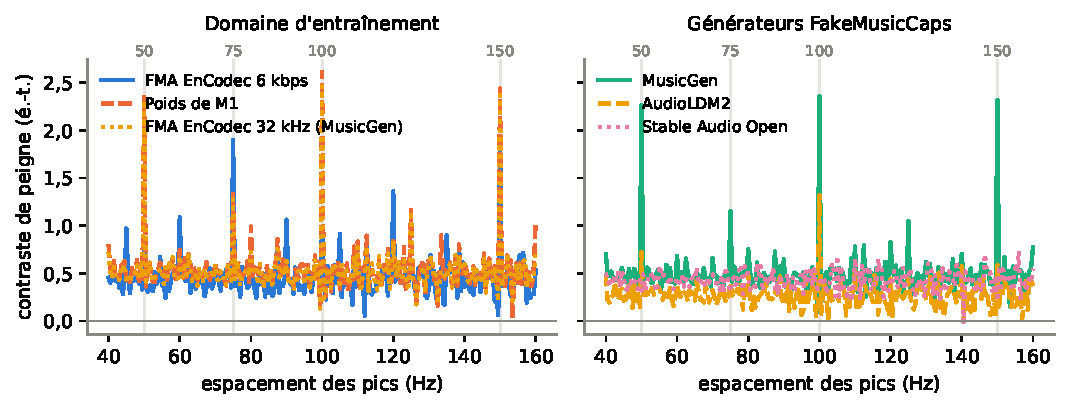
\includegraphics[width=\textwidth]{figures/fig_peigne_oracle.pdf}
    \caption{Contraste de peigne pour l'oracle MusicGen. À gauche, l'empreinte des reconstructions EnCodec
    24~kHz à 6~kbit/s (bleu), celle des reconstructions par l'EnCodec 32~kHz de MusicGen (pointillés) et les
    poids de l'oracle (tirets, « Poids de M1 » dans la légende). À droite, les générateurs, comme à la
    figure~\ref{fig:peigne}. 300 segments par série ; mesure descriptive, sans intervalle de confiance.}
    \label{fig:peigne_oracle}
\end{figure}

\begin{table}[h]
    \centering
    \footnotesize
    \setlength{\tabcolsep}{3.5pt}
    \begin{tabular}{lcccc}
        \toprule
        Générateur & M1 & Oracle [IC 95~\%] & Oracle $-$ M1 & Oracle $-$ M0 \\
        \midrule
        MusicGen          & 0,796 & 0,997 $[0{,}995~;~0{,}998]$ & $+0{,}200$ $[+0{,}183~;~+0{,}217]$ & $+0{,}250$ $[+0{,}221~;~+0{,}281]$ \\
        Stable Audio Open & 0,615 & 0,779 $[0{,}753~;~0{,}804]$ & $+0{,}165$ $[+0{,}137~;~+0{,}193]$ & $+0{,}173$ $[+0{,}126~;~+0{,}221]$ \\
        AudioLDM2         & 0,896 & 0,950 $[0{,}937~;~0{,}960]$ & $+0{,}053$ $[+0{,}036~;~+0{,}073]$ & $-0{,}022$ $[-0{,}037~;~-0{,}006]$ \\
        MusicLDM          & 0,899 & 0,920 $[0{,}902~;~0{,}935]$ & $+0{,}021$ $[+0{,}002~;~+0{,}041]$ & $+0{,}053$ $[+0{,}027~;~+0{,}081]$ \\
        Mustango          & 0,938 & 0,995 $[0{,}991~;~0{,}998]$ & $+0{,}057$ $[+0{,}044~;~+0{,}072]$ & $+0{,}045$ $[+0{,}036~;~+0{,}057]$ \\
        \midrule
        MusicGen $-$ autres & $-0{,}041$ & $+0{,}085$ $[+0{,}073~;~+0{,}100]$ & & \\
        \bottomrule
    \end{tabular}
    \caption{Oracle MusicGen contre M1 et M0, tous deux entraînés sur EnCodec 24~kHz à 6~kbit/s. Écarts
    appariés sur les mêmes segments, IC~95~\% par bootstrap groupé (1\,000 tirages).}
    \label{tab:oracle}
\end{table}

Sur MusicGen, l'oracle passe de 0,796 à 0,997 et détecte 99,5~\% des extraits au seuil fixé, contre 34~\%
pour M1 à 6~kbit/s. C'est aussi sur MusicGen qu'il dépasse le plus le détecteur trivial M0 ($+0{,}250$). L'écart
entre MusicGen et la moyenne des quatre autres générateurs change de signe : $+0{,}085$ $[+0{,}073~;~+0{,}100]$,
contre $-0{,}041$ pour M1 à 6~kbit/s (tableau~\ref{tab:oracle}).

L'oracle progresse pourtant sur les cinq générateurs. Mustango est détecté presque aussi bien que MusicGen
(0,995), et le gain le plus fort après MusicGen concerne Stable Audio Open ($+0{,}165$), qui ne laisse aucun
peigne. Une partie du gain ne vient donc pas de la cadence. Une explication possible, non testée, est le débit :
2,2~kbit/s dégrade davantage le signal que 6~kbit/s, et le détecteur peut apprendre des défauts plus généraux.
Cette étude ne sépare pas cadence et débit (section~\ref{sec:suite}). Deux observations complètent le tableau.
Le seuil fixé sur la validation donne 2~\% de faux positifs sur les réels du test, au lieu de 1~\%. L'oracle
détecte encore les reconstructions EnCodec 24~kHz à 6~kbit/s (AUC 0,907 $[0{,}886~;~0{,}925]$), ce qui est
compatible avec les multiples de 150~Hz communs aux deux peignes, sans que ce soit vérifié.

\paragraph{Verdict.} \textbf{Soutenu par un test direct, avec une réserve.} Le détecteur apprend le peigne de
la cadence de son codec d'entraînement : 75~Hz pour EnCodec 24~kHz, 50~Hz pour l'EnCodec de MusicGen.
L'oracle, dont la cadence est celle de MusicGen, détecte MusicGen mieux que la moyenne des autres générateurs
($+0{,}085$, contre au plus $+0{,}037$ pour M3 et $-0{,}041$ pour M1 à 6~kbit/s).
Réserve : l'oracle diffère aussi par son débit et progresse sur tous les générateurs ; la part due à la cadence
n'est pas isolée.

\subsection{Q3 : raccourcis de format}

\paragraph{Avant la chaîne : un raccourci total.} Prise seule comme score, chaque métadonnée de fichier sépare
les négatifs FMA des faux FakeMusicCaps (tableau~\ref{tab:meta}). Les fichiers FMA sont des MP3 de 30~s à 44,1
ou 48~kHz ; ceux de FakeMusicCaps des WAV mono de 10~s à 16~kHz. Un « détecteur » qui lirait la durée du fichier
aurait une AUC de 1. Entraîné sur les paires FMA, un détecteur de métadonnées n'apprendrait rien (réel et faux
héritent du même MP3) ; la séparabilité est donc mesurée directement sur les tests FakeMusicCaps. La chaîne
commune efface ces différences ; la question est ce qu'il en reste.

\begin{table}[h]
    \centering
    \small
    \begin{tabular}{lccc}
        \toprule
        Métadonnée & FMA (réels) & FakeMusicCaps (faux) & Séparabilité \\
        \midrule
        fréquence d'échantillonnage & 44,1 ou 48~kHz & 16~kHz & 1,000 \\
        débit & 128 à 320~kbit/s (MP3) & 512~kbit/s (WAV) & 1,000 \\
        durée & 30~s & 10 à 10,24~s & 1,000 \\
        canaux & mono ou stéréo & mono & 0,993 \\
        \bottomrule
    \end{tabular}
    \caption{Séparabilité ($\max(\mathrm{AUC}, 1-\mathrm{AUC})$) de chaque métadonnée prise seule comme
    score, identique pour les cinq générateurs. Sur les paires FMA, réel et faux héritent des métadonnées du
    même MP3 et la séparabilité vaut 0,5.}
    \label{tab:meta}
\end{table}

\paragraph{Après la chaîne : un raccourci résiduel.} M0, qui ne voit que des descripteurs triviaux calculés
après la chaîne, atteint 0,747 $[0{,}717~;~0{,}776]$ sur MusicGen ($p$ corrigé $= 0{,}008$), et ses
intervalles excluent 0,5 sur les cinq générateurs. M0 fait mieux que M1 sur AudioLDM2 (0,971 contre 0,896) et
sur Mustango à 12~kbit/s, et à peine moins bien ailleurs (figure~\ref{fig:m0m1}, tableau~\ref{tab:m1m0}). Sur
MusicGen, M1 dépasse M0 de $+0{,}049$ $[+0{,}016~;~+0{,}089]$ ($p$ corrigé $= 0{,}010$). Surtout, les deux
détecteurs s'accordent sur la difficulté des générateurs : Stable Audio Open puis MusicGen sont les plus durs
pour l'un comme pour l'autre, et les trois générateurs à VAE mel et vocodeur les plus faciles. Ce que M1 détecte
le mieux est aussi ce qui se distingue le plus de FMA par des propriétés de format.

\begin{figure}[h]
    \centering
    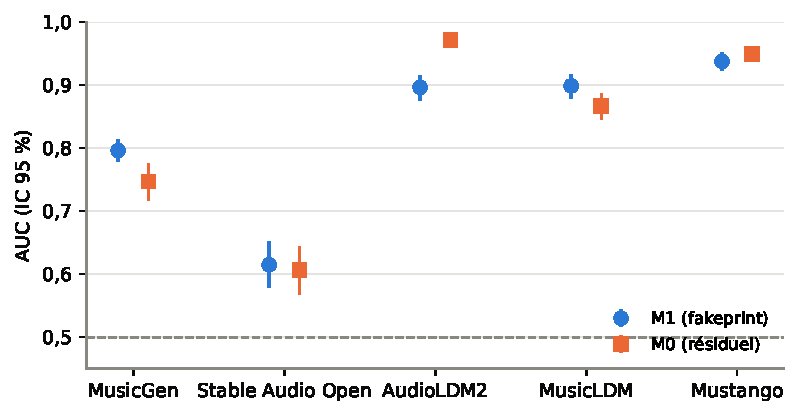
\includegraphics[width=0.78\textwidth]{figures/fig_m1_contre_m0.pdf}
    \caption{AUC de M1 (fakeprint) et de M0 (descripteurs triviaux) par générateur, détecteurs entraînés à
    6~kbit/s, IC~95~\% par bootstrap groupé. La ligne pointillée marque le hasard.}
    \label{fig:m0m1}
\end{figure}

\begin{table}[h]
    \centering
    \small
    \begin{tabular}{lcccc}
        \toprule
        & \multicolumn{2}{c}{6~kbit/s} & \multicolumn{2}{c}{12~kbit/s} \\
        \cmidrule(lr){2-3}\cmidrule(lr){4-5}
        Générateur & AUC M0 & M1 $-$ M0 [IC 95~\%] & AUC M0 & M1 $-$ M0 [IC 95~\%] \\
        \midrule
        MusicGen          & 0,747 & $+0{,}049$ $[+0{,}016~;~+0{,}089]$ & 0,701 & $+0{,}076$ $[+0{,}041~;~+0{,}117]$ \\
        Stable Audio Open & 0,607 & $+0{,}008$ $[-0{,}047~;~+0{,}067]$ & 0,611 & $-0{,}002$ $[-0{,}058~;~+0{,}061]$ \\
        AudioLDM2         & 0,971 & $-0{,}075$ $[-0{,}096~;~-0{,}053]$ & 0,969 & $-0{,}095$ $[-0{,}117~;~-0{,}070]$ \\
        MusicLDM          & 0,867 & $+0{,}032$ $[+0{,}005~;~+0{,}060]$ & 0,859 & $+0{,}032$ $[+0{,}005~;~+0{,}061]$ \\
        Mustango          & 0,950 & $-0{,}012$ $[-0{,}029~;~+0{,}005]$ & 0,950 & $-0{,}050$ $[-0{,}070~;~-0{,}030]$ \\
        \bottomrule
    \end{tabular}
    \caption{M0 et écart apparié M1 $-$ M0. M1 n'apporte un gain que sur MusicGen et MusicLDM ; il est
    battu par M0 sur AudioLDM2, et sur Mustango à 12~kbit/s.}
    \label{tab:m1m0}
\end{table}

\paragraph{Verdict.} \textbf{Oui}, mais c'est surtout une limite de notre protocole, pas une découverte sur les
détecteurs. Le raccourci vient de l'opposition entre deux bases (FMA et FakeMusicCaps), faute de vrais extraits
MusicCaps. Afchar et al. contrôlent ce risque à l'entraînement en appariant chaque piste réelle et sa
reconstruction \cite{afchar2024easy} ; notre entraînement fait de même, et le contrôle identité le confirme.
Le raccourci n'apparaît qu'au test.

\subsection{Q4 : robustesse aux attaques}

La figure~\ref{fig:attaques} et le tableau~\ref{tab:attaques} donnent les résultats. Sous un ralentissement de
10~\%, M1 perd 0,162 ; sous une accélération de 10~\%, il perd 0,297 et tombe au hasard (0,499), avec un taux de
détection de 0,3~\% au seuil fixé. L'AUC de M3 monte de 0,010 et de 0,020. La différence appariée des deux
variations vaut $-0{,}172$ $[-0{,}189~;~-0{,}154]$ sous $\times$0,9 et $-0{,}317$ $[-0{,}345~;~-0{,}287]$ sous
$\times$1,1 ($p$ corrigé $= 0{,}008$).

Le mécanisme est celui décrit par Dugelay et al. \cite{dugelay2026robustness} : un changement de vitesse de
facteur $a$ multiplie toutes les fréquences par $a$. Les pics espacés de 75~Hz le sont alors de 82,5~Hz sous
$\times$1,1 et ne tombent plus sur les poids linéaires de M1. En log-fréquence, c'est une translation, absorbée
par le maximum de la corrélation croisée de M3.

\begin{figure}[h]
    \centering
    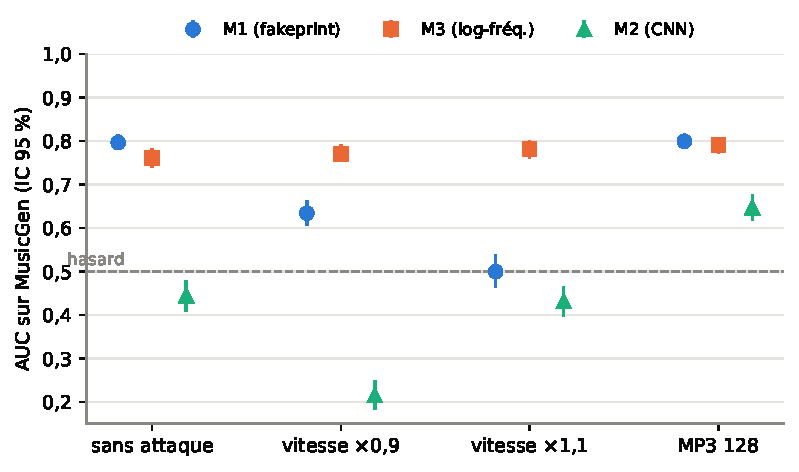
\includegraphics[width=0.78\textwidth]{figures/fig_attaques.pdf}
    \caption{AUC sur MusicGen sous attaque (détecteurs entraînés à 6~kbit/s ; M2 et M3 : graine~1).
    IC~95~\% par bootstrap groupé.}
    \label{fig:attaques}
\end{figure}

\begin{table}[h]
    \centering
    \small
    \begin{tabular}{llccc}
        \toprule
        Détecteur & Attaque & AUC & $\Delta$AUC [IC 95~\%] & TPR / FPR au seuil \\
        \midrule
        M1 & aucune      & 0,796 & ---                                    & 0,344 / 0,005 \\
           & vitesse $\times$0,9 & 0,634 & $-0{,}162$ $[-0{,}179~;~-0{,}144]$ & 0,197 / 0,007 \\
           & vitesse $\times$1,1 & 0,499 & $-0{,}297$ $[-0{,}324~;~-0{,}267]$ & 0,003 / 0,005 \\
           & MP3 128     & 0,799 & $+0{,}003$ $[+0{,}002~;~+0{,}004]$     & 0,364 / 0,005 \\
        \midrule
        M3 & aucune      & 0,761 & ---                                    & 0,379 / 0,016 \\
           & vitesse $\times$0,9 & 0,771 & $+0{,}010$ $[+0{,}003~;~+0{,}017]$ & 0,423 / 0,018 \\
           & vitesse $\times$1,1 & 0,781 & $+0{,}020$ $[+0{,}013~;~+0{,}028]$ & 0,395 / 0,023 \\
           & MP3 128     & 0,790 & $+0{,}029$ $[+0{,}025~;~+0{,}034]$     & 0,456 / 0,016 \\
        \midrule
        M2 & aucune      & 0,444 & ---                                    & 0,001 / 0,014 \\
           & vitesse $\times$0,9 & 0,215 & $-0{,}229$ $[-0{,}272~;~-0{,}185]$ & 0,047 / 0,325 \\
           & vitesse $\times$1,1 & 0,431 & $-0{,}013$ $[-0{,}065~;~+0{,}037]$ & 0,098 / 0,195 \\
           & MP3 128     & 0,646 & $+0{,}202$ $[+0{,}187~;~+0{,}219]$     & 0,037 / 0,020 \\
        \bottomrule
    \end{tabular}
    \caption{Attaques sur le test MusicGen. $\Delta$AUC apparié (attaque $-$ sans attaque) ; seuil fixé sur
    la validation, jamais réajusté.}
    \label{tab:attaques}
\end{table}

\paragraph{MP3.} Le MP3 à 128~kbit/s ne fait chuter ni M1 ($+0{,}003$) ni M3 ($+0{,}029$), et la différence
appariée penche en faveur de M3 ($-0{,}026$ $[-0{,}031~;~-0{,}022]$). Dugelay et al. n'ont pas testé la
compression \cite{dugelay2026robustness}. Afchar et al. observaient en revanche une forte chute de leur CNN sous
ré-encodage MP3 à 64~kbit/s \cite{afchar2024easy} ; ce résultat n'est pas retrouvé pour M1, mais le détecteur et
le débit diffèrent, et M2, notre CNN, réagit de façon erratique (voir ci-dessous).

\paragraph{Des attaques qui améliorent.} M3 gagne de 0,010 à 0,029 sous les trois attaques, et M2 gagne 0,202
sous MP3, alors qu'il s'inverse davantage sous ralentissement (0,215, avec un FPR qui passe de 1,4 à 32,5~\%).
Une attaque qui ne ferait qu'effacer des artefacts devrait faire baisser l'AUC. Une explication possible, non
testée ici, est que l'attaque transforme différemment les deux bases (MP3 d'origine contre WAV à 16~kHz) et
accentue ce qui les distingue.

\paragraph{Verdict.} \textbf{Répliqué dans un cadre différent}, avec une extension au MP3. Réserve : M3 est
entraîné avec une augmentation par vitesse ($\times$0,7 à $\times$1,4) qui couvre les attaques testées. Cette
étude ne sépare pas l'effet de l'architecture de celui de l'augmentation ; Dugelay et al. rapportent des
modèles entraînés avec et sans augmentation \cite{dugelay2026robustness}, nous non. Enfin, l'AUC de base
sur MusicGen contient une part de raccourci : le résultat montre que la décision de M1 est fragile, pas
exactement ce qu'elle perd.

\subsection{Synthèse des comparaisons principales}

\begin{table}[h]
    \centering
    \small
    \begin{tabularx}{\textwidth}{lYcc}
        \toprule
        & Comparaison & Valeur [IC 95~\%] & $p$ / $p$ Holm \\
        \midrule
        Q2 & AUC(M1, MusicGen) $-$ moyenne des quatre autres & $-0{,}041$ $[-0{,}052~;~-0{,}029]$ & 0,002 / 0,008 \\
        Q3 & AUC(M0, MusicGen) $-$ 0,5 & $+0{,}247$ $[+0{,}217~;~+0{,}276]$ & 0,002 / 0,008 \\
        Q3 & AUC(M1, MusicGen) $-$ AUC(M0, MusicGen) & $+0{,}049$ $[+0{,}016~;~+0{,}089]$ & 0,010 / 0,010 \\
        Q4 & \dAUC(M1) $-$ \dAUC(M3), vitesse $\times$1,1 & $-0{,}317$ $[-0{,}345~;~-0{,}287]$ & 0,002 / 0,008 \\
        \bottomrule
    \end{tabularx}
    \caption{Comparaisons principales (M1 et M0 entraînés à 6~kbit/s ; M3 graine~1). Tests bilatéraux,
    corrigés ensemble par Holm.}
    \label{tab:synthese}
\end{table}

\subsection{Autres mesures}

\paragraph{Le détecteur externe.} M4 (SONICS) obtient 0,820 sur Stable Audio Open, 0,735 sur MusicGen, 0,691
sur MusicLDM, 0,601 sur AudioLDM2 et 0,505 sur Mustango. Son profil est presque l'inverse de celui de M1 et de
M0. C'est cohérent avec un détecteur qui a appris d'autres artefacts, ou d'autres raccourcis, sur d'autres
données.

\paragraph{Faux positifs par genre.} Au seuil fixé, le taux de faux positifs reste faible dans tous les genres :
au plus 2~\% pour M1, au plus 6,1~\% pour M3 (« Experimental », 6 segments sur 98) et 8,3~\% dans le pire cas
(M2, graine~3, « Instrumental », 3 segments sur 36) (annexe~\ref{app:genre}). Avec 36 à 136 segments par genre,
ces mesures ne permettent pas d'exclure un biais modéré.

\paragraph{Les pires erreurs.} Les vingt réels que M1 juge les plus suspects viennent de 17 pistes, surtout
« Experimental » (5) et « Electronic » (4). Les faux MusicGen les plus manqués reçoivent un score quasi nul : le
détecteur se trompe avec assurance, ce qui est cohérent avec une décision fondée sur autre chose que
l'artefact.

% =====================================================================================================
\section{Apports et différences avec les papiers}
\label{sec:apports}

\begin{table}[h]
    \centering
    \small
    \begin{tabularx}{\textwidth}{lYY}
        \toprule
        & Papiers d'origine & Ce projet \\
        \midrule
        Entraînement & FMA \emph{medium} contre reconstructions Encodec, DAC, Musika, Griffin-Lim
        \cite{afchar2024easy} ; Suno~v5 contre FMA-small, Suno~v3.5 et Udio~v120 \cite{dugelay2026robustness} &
        FMA-small (2\,000 pistes) contre reconstructions EnCodec 24~kHz (6 et 12~kbit/s) uniquement ; EnCodec
        32~kHz de MusicGen pour l'oracle \\
        Générateurs testés & aucun \cite{afchar2024easy} ; 50 pistes MusicGen \cite{afchar2025challenges} ;
        Suno et Udio \cite{afchar2025fourier, dugelay2026robustness} & MusicGen, Stable Audio Open, AudioLDM2,
        MusicLDM, Mustango (FakeMusicCaps) \\
        Attaques & hauteur, étirement temporel, égalisation, réverbération, bruit, MP3/AAC/Opus 64~kbit/s
        \cite{afchar2024easy} ; vitesse, hauteur \cite{dugelay2026robustness} & vitesse $\times$0,9 et
        $\times$1,1, MP3 128~kbit/s \\
        Contrôle de raccourcis & réel et reconstruction appariés, même débit \cite{afchar2024easy} ; coupure
        à 16~kHz contre les artefacts MP3 \cite{afchar2025challenges} ; pas de contrôle explicite décrit
        \cite{dugelay2026robustness} & paires appariées, détecteur trivial M0, codec identité \\
        \bottomrule
    \end{tabularx}
    \caption{Cadre des papiers répliqués et cadre de ce projet.}
    \label{tab:cadres}
\end{table}

Ce qui est propre à ce projet :
\begin{itemize}
    \item le cadre « zéro donnée générée » appliqué au détecteur robuste (M3) ;
    \item l'évaluation sur les cinq générateurs de FakeMusicCaps, et sous MP3 à 128~kbit/s ;
    \item la lecture en fréquence des poids appris (peigne à 75~Hz contre 50~Hz), qui illustre l'explication
    de Fourier, et l'oracle MusicGen, qui la teste directement ;
    \item les contrôles « codec identité » et M0 : le premier montre que la chaîne ne fuit pas, le second
    qu'une grande part des AUC sur FakeMusicCaps tient à l'écart entre bases ;
    \item la méthode d'évaluation : bootstrap groupé par artiste ou légende, comparaisons appariées, plusieurs
    graines ;
    \item l'écart entre AUC et taux de détection au seuil fixé : AUC de 0,80 à 0,94, mais 2 à 34~\% de
    détection à 1~\% de faux positifs.
\end{itemize}

% =====================================================================================================
\section{Limites}
\label{sec:limites}

\begin{itemize}
    \item \textbf{Pas d'extraits réels MusicCaps.} Le contraste FakeMusicCaps mélange génération et domaine.
    C'est la limite qui conditionne toutes les autres lectures.
    \item Deux codecs d'entraînement seulement (EnCodec 24~kHz à deux débits ; EnCodec 32~kHz de MusicGen pour
    M1 seul) et 2\,000 pistes.
    \item Dans l'oracle, cadence et débit sont confondus (50~Hz et 2,2~kbit/s, contre 75~Hz et 6~kbit/s). Cette
    expérience a été définie après les premiers résultats.
    \item Attaques mesurées sur un seul générateur (MusicGen), avec une seule graine de M2 et M3, et pas sur le
    domaine d'entraînement, où l'effet de la vitesse serait mesuré sans raccourci.
    \item Dans M3, l'architecture log-fréquence et l'augmentation par vitesse sont confondues.
    \item La graine 3 de M2 et M3 (et M3 à 12~kbit/s, graine~2) a été entraînée dans un autre environnement
    logiciel et matériel que les autres (annexe~\ref{app:repro}). L'écart entre graines inclut donc aussi cet
    écart d'environnement.
\end{itemize}

% =====================================================================================================
\section{Suite}
\label{sec:suite}

\begin{enumerate}
    \item Séparer cadence et débit : entraîner M1 sur EnCodec 24~kHz à 3~kbit/s (4 dictionnaires, comme
    l'oracle, mais cadence de 75~Hz). Si MusicGen n'y progresse pas autant que dans l'oracle, la cadence
    explique la plus grande partie du gain.
    \item Opposer les faux à des réels \emph{du même domaine} (extraits MusicCaps réels, ou réels et faux issus
    d'une même chaîne), seule façon de mesurer le transfert sans raccourci.
    \item Entraîner M3 sans augmentation (ou M1 avec) pour séparer l'architecture de l'augmentation, et mesurer
    les attaques sur le domaine d'entraînement.
    \item Recalibrer les scores (mise à l'échelle par température) et rapporter les taux de détection à FPR
    fixé, plus proches d'un usage réel que l'AUC.
\end{enumerate}

\printbibliography[heading=bibintoc, title={Références}]

% =====================================================================================================
\newpage
\appendix

\section{Résultats par graine}
\label{app:graines}

\begin{table}[H]
    \centering
    \footnotesize
    \setlength{\tabcolsep}{4.5pt}
    \begin{tabular}{llccccccc}
        \toprule
        Détect. & Débit & Graine & MusicGen & S.\,A.\,Open & AudioLDM2 & MusicLDM & Mustango & MG $-$ autres \\
        \midrule
        M2 & 6  & 1 & 0,444 & 0,374 & 0,363 & 0,469 & 0,669 & $-0{,}025$ \\
        M2 & 6  & 2 & 0,611 & 0,498 & 0,606 & 0,626 & 0,790 & $-0{,}019$ \\
        M2 & 6  & 3 & 0,576 & 0,493 & 0,682 & 0,678 & 0,894 & $-0{,}111$ \\
        M2 & 12 & 1 & 0,454 & 0,448 & 0,316 & 0,534 & 0,721 & $-0{,}051$ \\
        M2 & 12 & 2 & 0,695 & 0,697 & 0,603 & 0,735 & 0,764 & $-0{,}004$ \\
        M2 & 12 & 3 & 0,421 & 0,199 & 0,331 & 0,576 & 0,585 & $-0{,}002$ \\
        \midrule
        M3 & 6  & 1 & 0,761 & 0,746 & 0,711 & 0,616 & 0,917 & $+0{,}014$ \\
        M3 & 6  & 2 & 0,767 & 0,744 & 0,715 & 0,620 & 0,923 & $+0{,}016$ \\
        M3 & 6  & 3 & 0,770 & 0,736 & 0,712 & 0,619 & 0,925 & $+0{,}022$ \\
        M3 & 12 & 1 & 0,762 & 0,722 & 0,697 & 0,602 & 0,904 & $+0{,}031$ \\
        M3 & 12 & 2 & 0,767 & 0,726 & 0,700 & 0,604 & 0,910 & $+0{,}032$ \\
        M3 & 12 & 3 & 0,765 & 0,714 & 0,691 & 0,604 & 0,900 & $+0{,}037$ \\
        \bottomrule
    \end{tabular}
    \caption{AUC par graine sur FakeMusicCaps (débit d'entraînement en kbit/s). Dernière colonne : écart
    MusicGen $-$ moyenne des quatre autres ; pour M3, les six intervalles excluent zéro. Sur leur domaine,
    toutes les graines atteignent 0,996 à 0,999.}
\end{table}

\section{Faux positifs par genre}
\label{app:genre}

\begin{table}[H]
    \centering
    \small
    \begin{tabular}{lccccccccc}
        \toprule
        Genre & $n$ & M0 & M1 & M2 g1 & M2 g2 & M2 g3 & M3 g1 & M3 g2 & M3 g3 \\
        \midrule
        Electronic    & 94  & 0,000 & 0,000 & 0,021 & 0,011 & 0,011 & 0,000 & 0,000 & 0,000 \\
        Experimental  & 98  & 0,031 & 0,020 & 0,020 & 0,031 & 0,010 & 0,061 & 0,061 & 0,041 \\
        Folk          & 118 & 0,000 & 0,000 & 0,008 & 0,000 & 0,000 & 0,008 & 0,008 & 0,008 \\
        Hip-Hop       & 78  & 0,013 & 0,000 & 0,013 & 0,000 & 0,026 & 0,000 & 0,000 & 0,000 \\
        Instrumental  & 36  & 0,028 & 0,000 & 0,000 & 0,000 & 0,083 & 0,028 & 0,028 & 0,028 \\
        International & 136 & 0,022 & 0,007 & 0,007 & 0,007 & 0,007 & 0,007 & 0,007 & 0,007 \\
        Pop           & 88  & 0,000 & 0,011 & 0,000 & 0,011 & 0,000 & 0,034 & 0,034 & 0,034 \\
        Rock          & 84  & 0,000 & 0,000 & 0,036 & 0,024 & 0,000 & 0,000 & 0,000 & 0,000 \\
        \bottomrule
    \end{tabular}
    \caption{Taux de faux positifs par genre sur les 732 segments réels du test FMA, au seuil fixé sur la
    validation (cible : 1~\%). $n$ : nombre de segments. Détecteurs entraînés à 6~kbit/s.}
\end{table}

\section{Reproductibilité et calcul}
\label{app:repro}

\paragraph{Code.} Le dépôt \texttt{musicdetect} contient la chaîne, les détecteurs, l'évaluation et le module
\texttt{musicdetect.analysis}, qui recalcule toutes les statistiques de ce rapport à partir des scores par
segment (\texttt{results/<tag>/scores/}) :
\begin{center}
\footnotesize\texttt{python -m musicdetect.analysis -{}-results results -{}-fma-index \dots{} -{}-fmc-index \dots{} -{}-out \dots}
\end{center}
Les figures et tableaux en sont tirés sans retouche ; le bootstrap utilise la graine 0. La figure du peigne
(figure~\ref{fig:peigne}) vient du module \texttt{musicdetect.peigne}, qui relit le modèle M1 et 300 segments
par source.

\paragraph{Déroulement.} M0, M1 et les graines 1 et 2 de M2 et M3 (sauf M3 à 12~kbit/s, graine~2) ont été
entraînés sur un ordinateur personnel, sur CPU (Python 3.13, scikit-learn 1.9.1, PyTorch 2.15, NumPy 2.5).
Des interruptions, dont un redémarrage par Windows Update, ont conduit à terminer sur Kaggle, en trois
sessions : une sur GPU T4 (3,8~h : graine~3 de M2 et M3 et M3 à 12~kbit/s graine~2, premières attaques de M2
et M3), deux sur CPU (0,8~h : réévaluation de M0 et M1 à 12~kbit/s et attaques de M1 ; 8,3~h : attaques des
trois détecteurs refaites avec enregistrement des scores par segment). L'image Kaggle fournissait Python 3.13,
NumPy 2.1, SciPy 1.16 et PyTorch 2.11 ; scikit-learn y a été imposé en version 1.9.1, car M0 et M1 sont
enregistrés par sérialisation (\emph{pickle}) et une autre version faisait échouer M1 ou rendait les scores de
M0 douteux. Une première évaluation de M0 à 12~kbit/s, faite avec une autre version de scikit-learn, a été
jetée et refaite avec la bonne version. L'oracle MusicGen a été calculé ensuite sur le même ordinateur, sur
CPU, avec transformers 5.22 : la reconstruction des 2\,000 pistes a pris 5~h~56.

\paragraph{Calcul et stockage.} Les attaques dominent le coût : l'aller-retour MP3 lance un encodeur par
segment. Sur CPU, une grille de trois attaques sur MusicGen a pris 70~min pour M1, 4,6~h pour M3 et 2,5~h
pour M2. Les segments occupent environ 13~Go ; modèles, scores et résultats environ 25~Mo.

\section{Glossaire}

\begin{description}
    \item[AUC] aire sous la courbe ROC ; probabilité qu'un faux tiré au hasard reçoive un score plus élevé
    qu'un réel tiré au hasard. 0,5 : hasard ; 1 : séparation parfaite ; sous 0,5 : décision inversée.
    \item[Bootstrap groupé] rééchantillonnage avec remise de groupes entiers (artistes, légendes) plutôt que
    de segments, pour respecter leur dépendance.
    \item[Codec neuronal] réseau qui compresse le signal en jetons discrets et le reconstruit ; la
    quantification vectorielle résiduelle empile plusieurs dictionnaires, chacun codant l'erreur du précédent.
    \item[Contraste de peigne] valeur moyenne d'un profil spectral, en écarts-types, aux multiples d'un
    espacement donné ; mesure descriptive définie pour cette analyse.
    \item[ECE] erreur de calibration : écart moyen entre le score annoncé et la fréquence réelle des faux.
    \item[Fakeprint] résidu du spectre moyen au-dessus de son enveloppe inférieure ; il isole les pics fins
    et réguliers laissés par un décodeur.
    \item[FPR, TPR] taux de faux positifs (réels déclarés faux) et taux de détection (faux déclarés faux) à
    un seuil donné.
    \item[Holm] correction des tests multiples : les $m$ valeurs $p$ triées sont comparées à
    $\alpha/m, \alpha/(m-1), \dots$, ce qui contrôle le risque de faux positif sur l'ensemble des tests.
    \item[Raccourci] indice qui sépare les classes dans les données d'étude sans être la propriété visée
    (ici : format, bande passante, durée).
    \item[Test apparié] comparaison de deux mesures sur les mêmes exemples, qui élimine la variabilité due
    aux exemples eux-mêmes.
\end{description}

\end{document}
